\documentclass[aspectratio=1610]{beamer}

\usetheme{KTH}

% remove this if using XeLaTeX or LuaLaTeX
\usepackage[utf8]{inputenc}

\usepackage{wrapfig}
\usepackage{subcaption}

\usepackage{tikz}

\usepackage[export]{adjustbox}

\usepackage{keyval}
\usepackage{ifthen}
%====================================
%emphasize vertices --> switch and emph style (e.g. thick,black)
%====================================
\makeatletter
% Standard Values for Parameters
\newcommand{\tikzcuboid@shiftx}{0}
\newcommand{\tikzcuboid@shifty}{0}
\newcommand{\tikzcuboid@dimx}{3}
\newcommand{\tikzcuboid@dimy}{3}
\newcommand{\tikzcuboid@dimz}{3}
\newcommand{\tikzcuboid@scale}{1}
\newcommand{\tikzcuboid@densityx}{1}
\newcommand{\tikzcuboid@densityy}{1}
\newcommand{\tikzcuboid@densityz}{1}
\newcommand{\tikzcuboid@rotation}{0}
\newcommand{\tikzcuboid@anglex}{0}
\newcommand{\tikzcuboid@angley}{90}
\newcommand{\tikzcuboid@anglez}{225}
\newcommand{\tikzcuboid@scalex}{1}
\newcommand{\tikzcuboid@scaley}{1}
\newcommand{\tikzcuboid@scalez}{sqrt(0.5)}
\newcommand{\tikzcuboid@linefront}{black}
\newcommand{\tikzcuboid@linetop}{black}
\newcommand{\tikzcuboid@lineright}{black}
\newcommand{\tikzcuboid@fillfront}{white}
\newcommand{\tikzcuboid@filltop}{white}
\newcommand{\tikzcuboid@fillright}{white}
\newcommand{\tikzcuboid@shaded}{N}
\newcommand{\tikzcuboid@shadecolor}{black}
\newcommand{\tikzcuboid@shadeperc}{25}
\newcommand{\tikzcuboid@emphedge}{N}
\newcommand{\tikzcuboid@emphstyle}{thick}

% Definition of Keys
\define@key{tikzcuboid}{shiftx}[\tikzcuboid@shiftx]{\renewcommand{\tikzcuboid@shiftx}{#1}}
\define@key{tikzcuboid}{shifty}[\tikzcuboid@shifty]{\renewcommand{\tikzcuboid@shifty}{#1}}
\define@key{tikzcuboid}{dimx}[\tikzcuboid@dimx]{\renewcommand{\tikzcuboid@dimx}{#1}}
\define@key{tikzcuboid}{dimy}[\tikzcuboid@dimy]{\renewcommand{\tikzcuboid@dimy}{#1}}
\define@key{tikzcuboid}{dimz}[\tikzcuboid@dimz]{\renewcommand{\tikzcuboid@dimz}{#1}}
\define@key{tikzcuboid}{scale}[\tikzcuboid@scale]{\renewcommand{\tikzcuboid@scale}{#1}}
\define@key{tikzcuboid}{densityx}[\tikzcuboid@densityx]{\renewcommand{\tikzcuboid@densityx}{#1}}
\define@key{tikzcuboid}{densityy}[\tikzcuboid@densityy]{\renewcommand{\tikzcuboid@densityy}{#1}}
\define@key{tikzcuboid}{densityz}[\tikzcuboid@densityz]{\renewcommand{\tikzcuboid@densityz}{#1}}
\define@key{tikzcuboid}{rotation}[\tikzcuboid@rotation]{\renewcommand{\tikzcuboid@rotation}{#1}}
\define@key{tikzcuboid}{anglex}[\tikzcuboid@anglex]{\renewcommand{\tikzcuboid@anglex}{#1}}
\define@key{tikzcuboid}{angley}[\tikzcuboid@angley]{\renewcommand{\tikzcuboid@angley}{#1}}
\define@key{tikzcuboid}{anglez}[\tikzcuboid@anglez]{\renewcommand{\tikzcuboid@anglez}{#1}}
\define@key{tikzcuboid}{scalex}[\tikzcuboid@scalex]{\renewcommand{\tikzcuboid@scalex}{#1}}
\define@key{tikzcuboid}{scaley}[\tikzcuboid@scaley]{\renewcommand{\tikzcuboid@scaley}{#1}}
\define@key{tikzcuboid}{scalez}[\tikzcuboid@scalez]{\renewcommand{\tikzcuboid@scalez}{#1}}
\define@key{tikzcuboid}{linefront}[\tikzcuboid@linefront]{\renewcommand{\tikzcuboid@linefront}{#1}}
\define@key{tikzcuboid}{linetop}[\tikzcuboid@linetop]{\renewcommand{\tikzcuboid@linetop}{#1}}
\define@key{tikzcuboid}{lineright}[\tikzcuboid@lineright]{\renewcommand{\tikzcuboid@lineright}{#1}}
\define@key{tikzcuboid}{fillfront}[\tikzcuboid@fillfront]{\renewcommand{\tikzcuboid@fillfront}{#1}}
\define@key{tikzcuboid}{filltop}[\tikzcuboid@filltop]{\renewcommand{\tikzcuboid@filltop}{#1}}
\define@key{tikzcuboid}{fillright}[\tikzcuboid@fillright]{\renewcommand{\tikzcuboid@fillright}{#1}}
\define@key{tikzcuboid}{shaded}[\tikzcuboid@shaded]{\renewcommand{\tikzcuboid@shaded}{#1}}
\define@key{tikzcuboid}{shadecolor}[\tikzcuboid@shadecolor]{\renewcommand{\tikzcuboid@shadecolor}{#1}}
\define@key{tikzcuboid}{shadeperc}[\tikzcuboid@shadeperc]{\renewcommand{\tikzcuboid@shadeperc}{#1}}
\define@key{tikzcuboid}{emphedge}[\tikzcuboid@emphedge]{\renewcommand{\tikzcuboid@emphedge}{#1}}
\define@key{tikzcuboid}{emphstyle}[\tikzcuboid@emphstyle]{\renewcommand{\tikzcuboid@emphstyle}{#1}}
% Commands
\newcommand{\tikzcuboid}[1]{
    \setkeys{tikzcuboid}{#1} % Process Keys passed to command
    \pgfmathsetmacro{\vectorxx}{\tikzcuboid@scalex*cos(\tikzcuboid@anglex)}
    \pgfmathsetmacro{\vectorxy}{\tikzcuboid@scalex*sin(\tikzcuboid@anglex)}
    \pgfmathsetmacro{\vectoryx}{\tikzcuboid@scaley*cos(\tikzcuboid@angley)}
    \pgfmathsetmacro{\vectoryy}{\tikzcuboid@scaley*sin(\tikzcuboid@angley)}
    \pgfmathsetmacro{\vectorzx}{\tikzcuboid@scalez*cos(\tikzcuboid@anglez)}
    \pgfmathsetmacro{\vectorzy}{\tikzcuboid@scalez*sin(\tikzcuboid@anglez)}
    \begin{scope}[xshift=\tikzcuboid@shiftx, yshift=\tikzcuboid@shifty, scale=\tikzcuboid@scale, rotate=\tikzcuboid@rotation, x={(\vectorxx,\vectorxy)}, y={(\vectoryx,\vectoryy)}, z={(\vectorzx,\vectorzy)}]
    \pgfmathsetmacro{\steppingx}{1/\tikzcuboid@densityx}
    \pgfmathsetmacro{\steppingy}{1/\tikzcuboid@densityy}
    \pgfmathsetmacro{\steppingz}{1/\tikzcuboid@densityz}
    \newcommand{\dimx}{\tikzcuboid@dimx}
    \newcommand{\dimy}{\tikzcuboid@dimy}
    \newcommand{\dimz}{\tikzcuboid@dimz}
    \pgfmathsetmacro{\secondx}{2*\steppingx}
    \pgfmathsetmacro{\secondy}{2*\steppingy}
    \pgfmathsetmacro{\secondz}{2*\steppingz}
    \foreach \x in {\steppingx,\secondx,...,\dimx}
    {   \foreach \y in {\steppingy,\secondy,...,\dimy}
        {   \pgfmathsetmacro{\lowx}{(\x-\steppingx)}
            \pgfmathsetmacro{\lowy}{(\y-\steppingy)}
            \filldraw[fill=\tikzcuboid@fillfront,draw=\tikzcuboid@linefront] (\lowx,\lowy,\dimz) -- (\lowx,\y,\dimz) -- (\x,\y,\dimz) -- (\x,\lowy,\dimz) -- cycle;

        }
    }
    \foreach \x in {\steppingx,\secondx,...,\dimx}
    {   \foreach \z in {\steppingz,\secondz,...,\dimz}
        {   \pgfmathsetmacro{\lowx}{(\x-\steppingx)}
            \pgfmathsetmacro{\lowz}{(\z-\steppingz)}
            \filldraw[fill=\tikzcuboid@filltop,draw=\tikzcuboid@linetop] (\lowx,\dimy,\lowz) -- (\lowx,\dimy,\z) -- (\x,\dimy,\z) -- (\x,\dimy,\lowz) -- cycle;
        }
    }
    \foreach \y in {\steppingy,\secondy,...,\dimy}
    {   \foreach \z in {\steppingz,\secondz,...,\dimz}
        {   \pgfmathsetmacro{\lowy}{(\y-\steppingy)}
            \pgfmathsetmacro{\lowz}{(\z-\steppingz)}
            \filldraw[fill=\tikzcuboid@fillright,draw=\tikzcuboid@lineright] (\dimx,\lowy,\lowz) -- (\dimx,\lowy,\z) -- (\dimx,\y,\z) -- (\dimx,\y,\lowz) -- cycle;
        }
    }
    \ifthenelse{\equal{\tikzcuboid@emphedge}{Y}}%
        {\draw[\tikzcuboid@emphstyle](0,\dimy,0) -- (\dimx,\dimy,0) -- (\dimx,\dimy,\dimz) -- (0,\dimy,\dimz) -- cycle;%
        \draw[\tikzcuboid@emphstyle] (0,0,\dimz) -- (0,\dimy,\dimz) -- (\dimx,\dimy,\dimz) -- (\dimx,0,\dimz) -- cycle;%
        \draw[\tikzcuboid@emphstyle](\dimx,0,0) -- (\dimx,\dimy,0) -- (\dimx,\dimy,\dimz) -- (\dimx,0,\dimz) -- cycle;%
        }%
        {}
    \end{scope}
}

\makeatother



\begin{document}

\startpage
%%%%%%%%%%%%%%%%%%%%%%%%%%%%%%%%%%%%%%%%%%%%%%%%%%%%%%%%%%%%
\begin{frame}

  \vspace{0.02\textheight}
  
  \begin{Large}
    Newspaper article segmentation \\
    using Mask R-CNN and Sentence-BERT
  \end{Large}



  \vspace{0.1\textheight}

  \begin{small}
    \textit{Gustav Henning}
  \end{small}
\end{frame}


\normalpage
%%%%%%%%%%%%%%%%%%%%%%%%%%%%%%%%%%%%%%%%%%%%%%%%%%%%%%%%%%%%
\begin{frame}
  \frametitle{Why newspaper article segmentation?}

  \begin{block}{Focus on digitalization of documents}
    \begin{itemize}
    \item Pages are scanned on an image level
    \item Optical Character Recognition extracts boxes of text
    \item Document layout analysis, reading order, article segmentation remains a challenge
    \end{itemize}
  \end{block}

\end{frame}
\normalpage


%%%%%%%%%%%%%%%%%%%%%%%%%%%%%%%%%%%%%%%%%%%%%%%%%%%%%%%%%%%%
\begin{frame}
\begin{figure}
\centering
\begin{subfigure}{.5\textwidth}
  \centering
  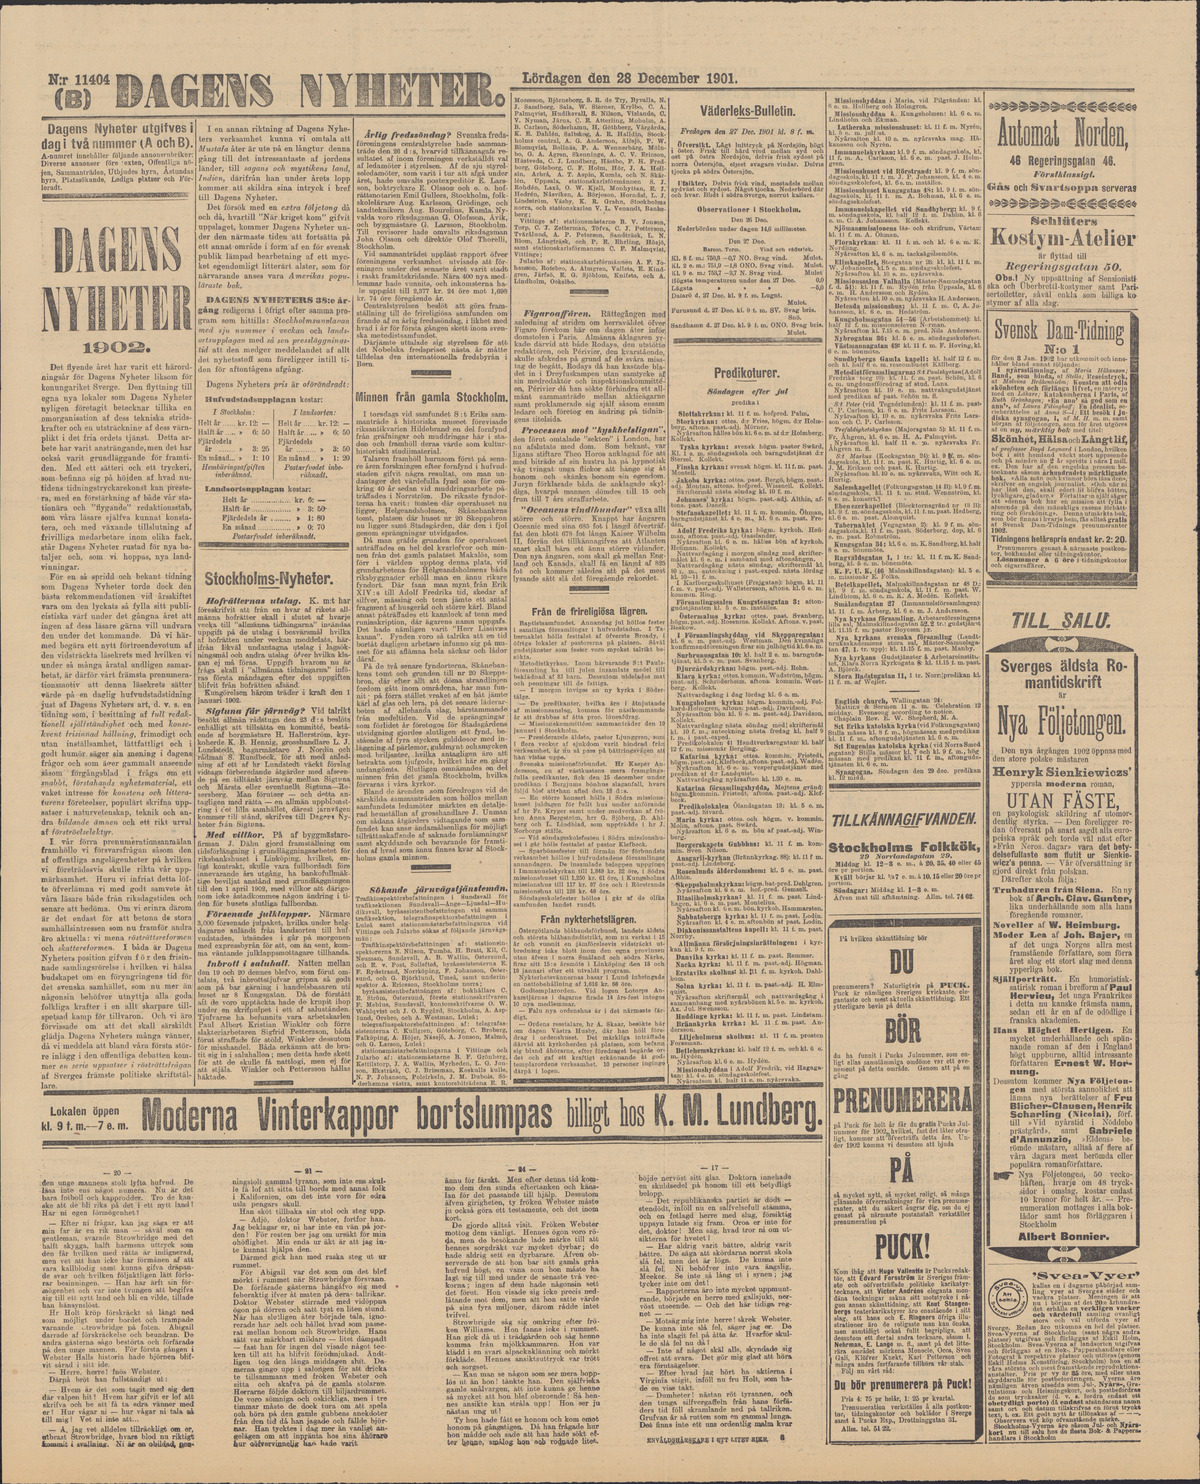
\includegraphics[max size={0.95\textwidth}{0.95\textheight}]{figures/1901.jpg}
  \caption{A newspaper page from 1901.}
  \label{fig:raw1901}
\end{subfigure}%
\begin{subfigure}{.5\textwidth}
  \centering
  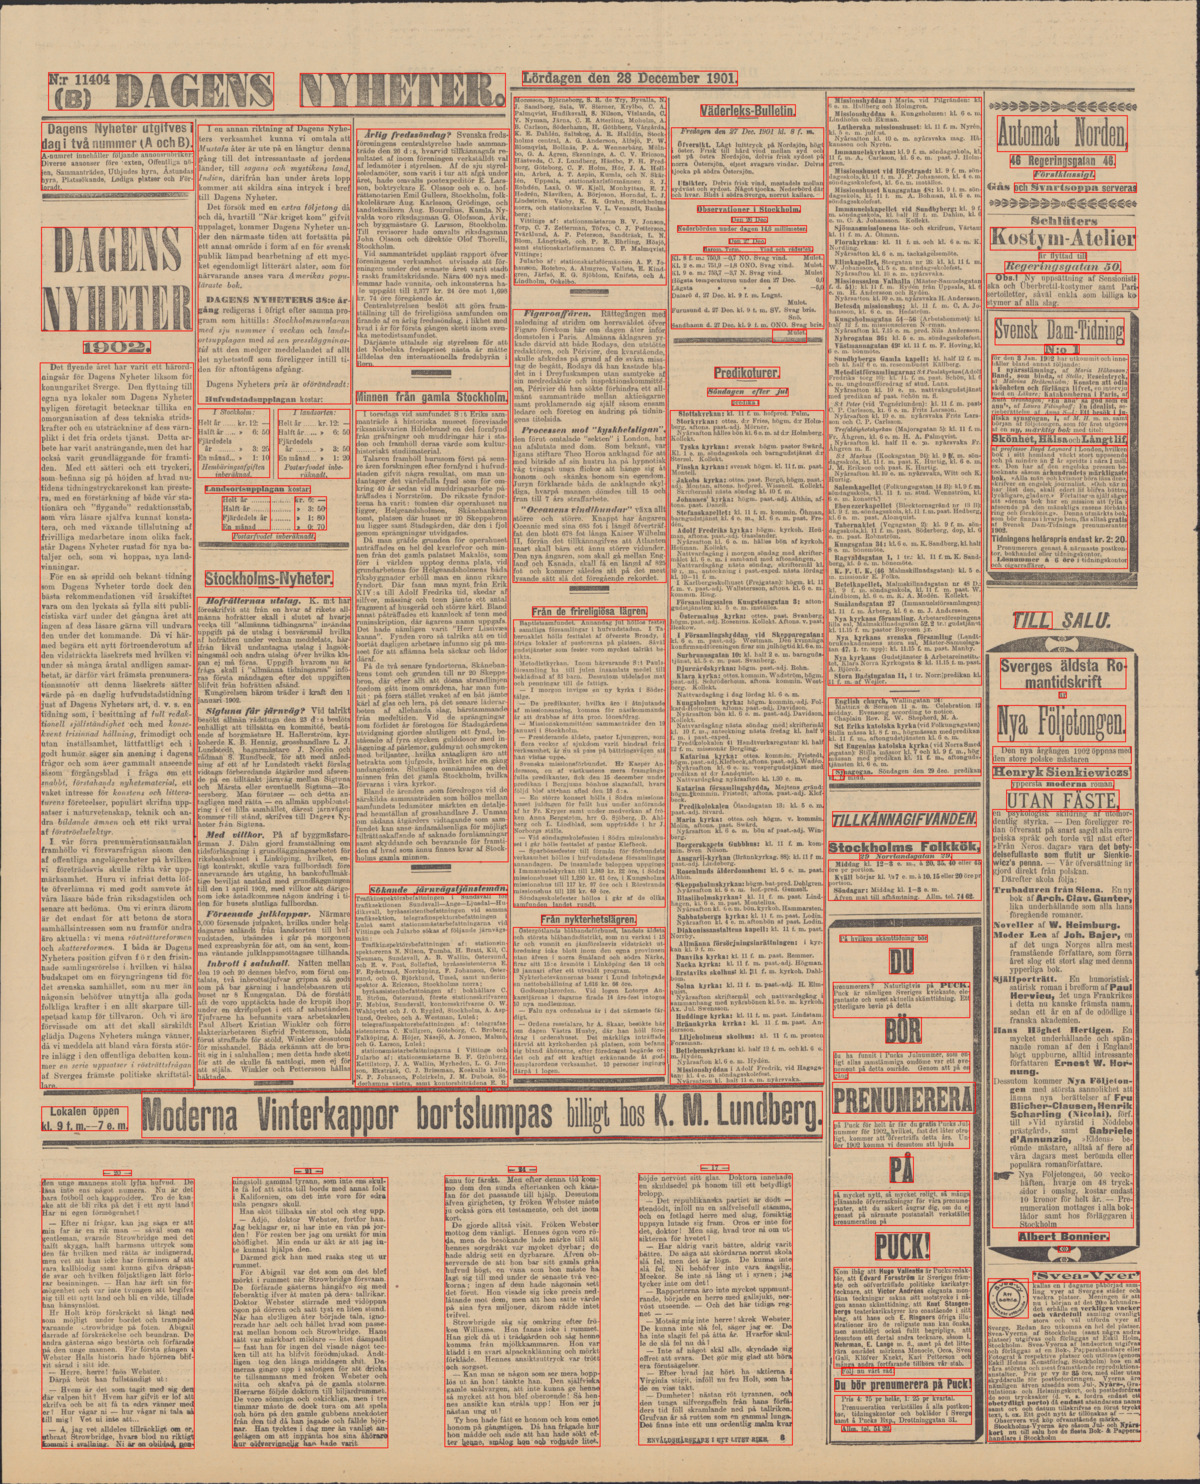
\includegraphics[max size={0.95\textwidth}{0.95\textheight}]{figures/1901-ocr.jpg}
  \caption{OCR bounding boxes visualized in red.}
  \label{fig:ocr1901}
\end{subfigure}
\label{fig:1901}
\end{figure}

\end{frame}
\normalpage

%%%%%%%%%%%%%%%%%%%%%%%%%%%%%%%%%%%%%%%%%%%%%%%%%%%%%%%%%%%%
\begin{frame}
  \frametitle{Problems and goals}

  \begin{Large}
    Problem statement
  \end{Large}

  \begin{small}
  How well can neural networks, developed for object detection and
segmentation of real-world objects, perform in the domain of news article
segmentation?
  \break
  \end{small}

  \begin{Large}
    Goals 
  \end{Large}


  \begin{small}
    \begin{itemize}
    \item Do multimodal neural network architectures outperform unimodal neural
network architectures, using image and text input as opposed to only
using image input, in the field of instance segmentation?
    \item Is there a difference in how well multimodal neural network architectures
perform in periods of changing typographic design as opposed to
unimodal neural network architectures?
    \end{itemize}
  \end{small}

\end{frame}
\normalpage

%%%%%%%%%%%%%%%%%%%%%%%%%%%%%%%%%%%%%%%%%%%%%%%%%%%%%%%%%%%%
\begin{frame}
  \frametitle{What is Mask R-CNN?}
\begin{figure}
\centering
\begin{subfigure}{0.8\textwidth}
  \centering
  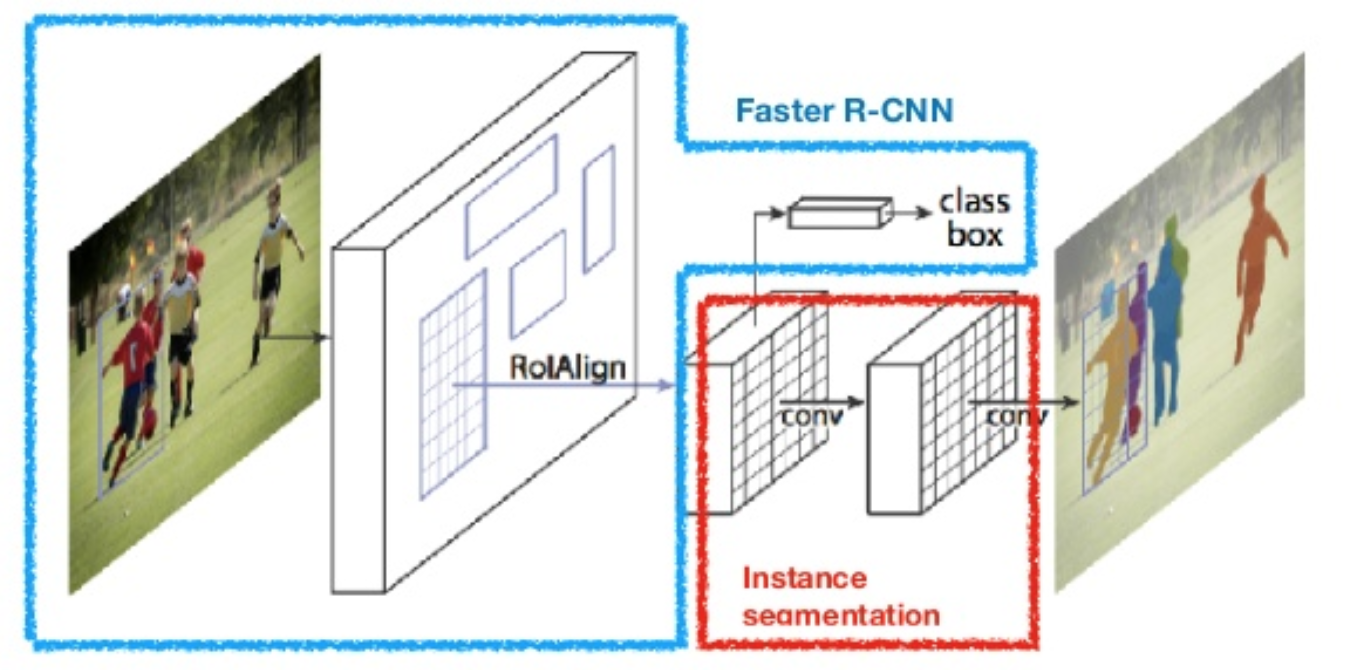
\includegraphics[max size={0.9\textwidth}{0.9\textheight}]{figures/mask-rcnn.png}
  \caption{Mask R-CNN architecture. [He et al 2017]}
  \label{fig:submaskrcnn}
\end{subfigure}%
\label{fig:maskrcnn}
\end{figure}
\end{frame}
\normalpage

%%%%%%%%%%%%%%%%%%%%%%%%%%%%%%%%%%%%%%%%%%%%%%%%%%%%%%%%%%%%
\begin{frame}
\begin{figure}
\centering
\begin{subfigure}{0.9\textwidth}
  \centering
  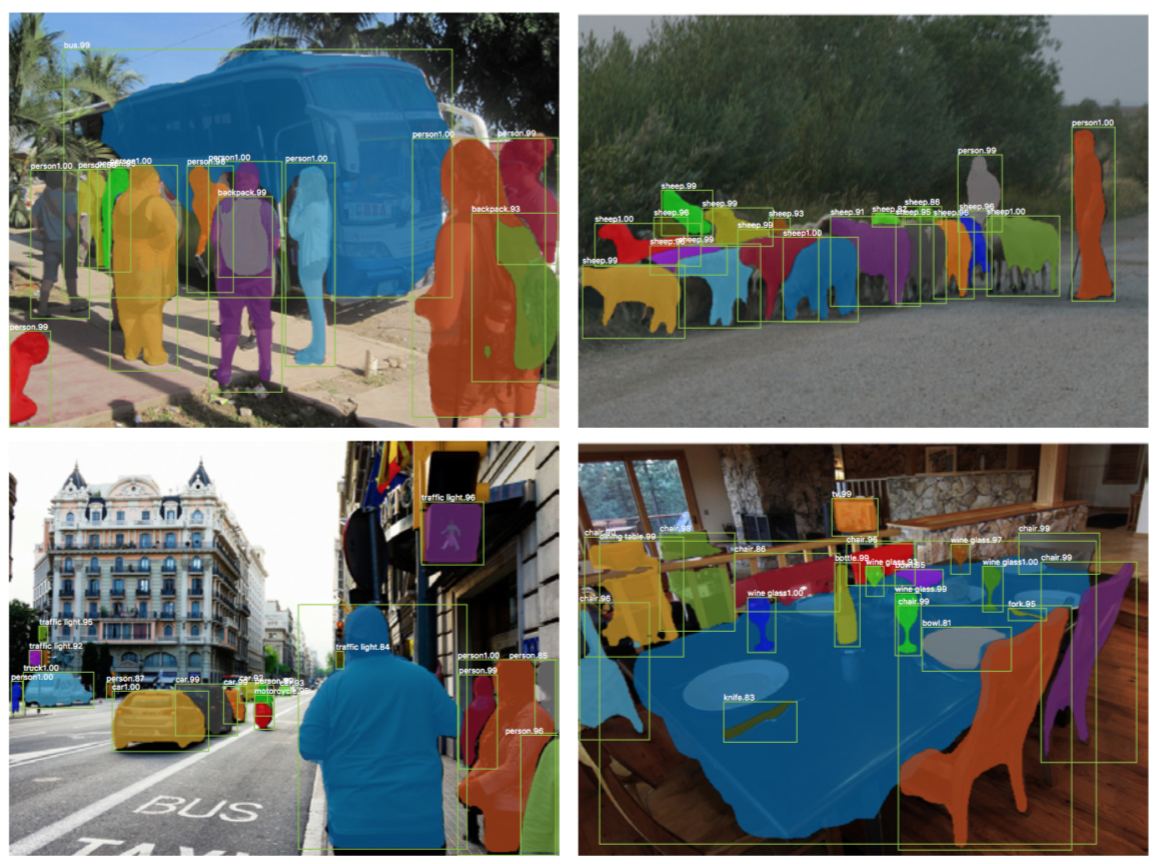
\includegraphics[max size={0.9\textwidth}{0.9\textheight}]{figures/mask-rcnn-examples.png}
  \caption{Mask R-CNN output for MS COCO (Common objects in Context). [He et al 2017]}
  \label{fig:submscoco}
\end{subfigure}%
\label{fig:mscoco}
\end{figure}
\end{frame}
\normalpage

%%%%%%%%%%%%%%%%%%%%%%%%%%%%%%%%%%%%%%%%%%%%%%%%%%%%%%%%%%%%
\begin{frame}
  \frametitle{Feature Pyramid Network}
wow
\end{frame}
\normalpage

%%%%%%%%%%%%%%%%%%%%%%%%%%%%%%%%%%%%%%%%%%%%%%%%%%%%%%%%%%%%
\begin{frame}
  \frametitle{Architecture modularity and pretrained weights}
wow
\end{frame}
\normalpage

%%%%%%%%%%%%%%%%%%%%%%%%%%%%%%%%%%%%%%%%%%%%%%%%%%%%%%%%%%%%
\begin{frame}
  \frametitle{What is (Sentence-) BERT?}
wow
\end{frame}
\normalpage

%%%%%%%%%%%%%%%%%%%%%%%%%%%%%%%%%%%%%%%%%%%%%%%%%%%%%%%%%%%%
\begin{frame}
  \frametitle{Sentence transformers used in this thesis}
table
\end{frame}
\normalpage


%%%%%%%%%%%%%%%%%%%%%%%%%%%%%%%%%%%%%%%%%%%%%%%%%%%%%%%%%%%%
\begin{frame}
  \frametitle{How do we combine the visual and textual modalities?}
\begin{tikzpicture}

    \tikzcuboid{%
        shiftx=12cm,%
        shifty=8cm,%
        scale=0.6,%
        rotation=0,%
        densityx=2,%
        densityy=1,%
        densityz=1,%
        dimx=1,%
        dimy=6,%
        dimz=6,%
        linefront=red!25!white,%
        linetop=red!50!white,%
        lineright=red!25!black,%
        fillfront=red!25!white,%
        filltop=red!50!white,%
        fillright=red!75!white,%
        emphedge=Y,%
        emphstyle=very thick,
    }
    \tikzcuboid{%
        shiftx=14cm,%
        shifty=8cm,%
        scale=0.6,%
        rotation=0,%
        densityx=2,%
        densityy=1,%
        densityz=1,%
        dimx=1,%
        dimy=6,%
        dimz=6,%
        linefront=green!25!white,%
        linetop=green!50!white,%
        lineright=green!25!black,%
        fillfront=green!25!white,%
        filltop=green!50!white,%
        fillright=green!75!white,%
        emphedge=Y,%
        emphstyle=very thick,
    }

    \tikzcuboid{%
        shiftx=16cm,%
        shifty=8cm,%
        scale=0.6,%
        rotation=0,%
        densityx=2,%
        densityy=1,%
        densityz=1,%
        dimx=1,%
        dimy=6,%
        dimz=6,%
        linefront=blue!25!white,%
        linetop=blue!50!white,%
        lineright=blue!25!black,%
        fillfront=blue!25!white,%
        filltop=blue!50!white,%
        fillright=blue!75!white,%
        emphedge=Y,%
        emphstyle=very thick,
    }

    \tikzcuboid{%
        shiftx=18cm,%
        shifty=8cm,%
        scale=0.6,%
        rotation=0,%
        densityx=2,%
        densityy=1,%
        densityz=1,%
        dimx=1,%
        dimy=6,%
        dimz=6,%
        linefront=black!25!white,%
        linetop=black!50!white,%
        lineright=black!25!black,%
        fillfront=black!25!white,%
        filltop=black!50!white,%
        fillright=black!75!white,%
        emphedge=Y,%
        emphstyle=very thick,
    }

    \tikzcuboid{%
        shiftx=20cm,%
        shifty=8cm,%
        scale=0.6,%
        rotation=0,%
        densityx=2,%
        densityy=1,%
        densityz=1,%
        dimx=1,%
        dimy=6,%
        dimz=6,%
        linefront=black!25!white,%
        linetop=black!50!white,%
        lineright=black!25!black,%
        fillfront=black!25!white,%
        filltop=black!50!white,%
        fillright=black!75!white,%
        emphedge=Y,%
        emphstyle=very thick,
    }

    \tikzcuboid{%
        shiftx=22cm,%
        shifty=8cm,%
        scale=0.6,%
        rotation=0,%
        densityx=2,%
        densityy=1,%
        densityz=1,%
        dimx=1,%
        dimy=6,%
        dimz=6,%
        linefront=black!25!white,%
        linetop=black!50!white,%
        lineright=black!25!black,%
        fillfront=black!25!white,%
        filltop=black!50!white,%
        fillright=black!75!white,%
        emphedge=Y,%
        emphstyle=very thick,
    }
\end{tikzpicture}
\begin{small}

3 native RGB channels + 3 text embedding channels
\end{small}
\end{frame}
\normalpage


%%%%%%%%%%%%%%%%%%%%%%%%%%%%%%%%%%%%%%%%%%%%%%%%%%%%%%%%%%%%
\begin{frame}
  \frametitle{Datasets created in this thesis}

\begin{tikzpicture}
 
\node[rectangle,
    draw = lightgray,
    text = black,
    fill = orange!30!,
    minimum width = 6cm, 
    minimum height = 1cm] (r) at (0,0) {\small Train(N=510)};


\node[rectangle,
    draw = lightgray,
    text = black,
    fill = blue!30!,
    minimum width = 2cm, 
    minimum height = 1cm] (r) at (5,0) {\small Test(N=109)};

\node[rectangle,
    draw = lightgray,
    text = black,
    fill = green!30!,
    minimum width = 2cm, 
    minimum height = 1cm] (r) at (8,0) {\small Validation(N=111)};

\node[rectangle,
    draw = white,
    text = black,
    fill = white!30!,
    minimum width = 2cm, 
    minimum height = 1cm] (r) at (11,0) {\small DN 2010-2020};


\node[rectangle,
    draw = lightgray,
    text = black,
    fill = blue!30!,
    minimum width = 2cm, 
    minimum height = 1cm] (r) at (5,-1) {\small Test(N=195)};


\node[rectangle,
    draw = white,
    text = black,
    fill = white!30!,
    minimum width = 2cm, 
    minimum height = 1cm] (r) at (11,-1) {\small DN SvD 2001-2004};

\node[rectangle,
    draw = lightgray,
    text = black,
    fill = blue!30!,
    minimum width = 2cm, 
    minimum height = 1cm] (r) at (5,-2) {\small Test(N=200)};


\node[rectangle,
    draw = white,
    text = black,
    fill = white!30!,
    minimum width = 2cm, 
    minimum height = 1cm] (r) at (11,-2) {AB EX 2001-2004};
\end{tikzpicture}

\begin{small}
Morning newspapers: DN = Dagens Nyheter, SvD = Svenska Dagbladet

Evening newspapers: AB = Aftonbladet, EX = Expressen


DN 2010-2020 is split (70/15/15) using random sampling.
\end{small}
\end{frame}
\normalpage

%%%%%%%%%%%%%%%%%%%%%%%%%%%%%%%%%%%%%%%%%%%%%%%%%%%%%%%%%%%%
\begin{frame}
  \frametitle{Labeling Strategy}
Classes, caveats
\end{frame}
\normalpage


%%%%%%%%%%%%%%%%%%%%%%%%%%%%%%%%%%%%%%%%%%%%%%%%%%%%%%%%%%%%
\begin{frame}
  \frametitle{Experiments}
Unimodal vs multimodal

impact of class labels

impact of dataset size

\end{frame}
\normalpage


%%%%%%%%%%%%%%%%%%%%%%%%%%%%%%%%%%%%%%%%%%%%%%%%%%%%%%%%%%%%
\begin{frame}
  \frametitle{Performance Metrics}
wow
\end{frame}
\normalpage


%%%%%%%%%%%%%%%%%%%%%%%%%%%%%%%%%%%%%%%%%%%%%%%%%%%%%%%%%%%%
\begin{frame}
  \frametitle{Results}
wow
\end{frame}
\normalpage

%%%%%%%%%%%%%%%%%%%%%%%%%%%%%%%%%%%%%%%%%%%%%%%%%%%%%%%%%%%%
\begin{frame}
  \frametitle{Discussion and conclusion}
wow
\end{frame}
\normalpage

%%%%%%%%%%%%%%%%%%%%%%%%%%%%%%%%%%%%%%%%%%%%%%%%%%%%%%%%%%%%
\begin{frame}
  \frametitle{Example of OCR, Visualized embedding, Best model prediction}
wow
\end{frame}
\normalpage

%%%%%%%%%%%%%%%%%%%%%%%%%%%%%%%%%%%%%%%%%%%%%%%%%%%%%%%%%%%%
\begin{frame}
  \frametitle{Example of OCR, Visualized embedding, Best model prediction}
wow
\end{frame}
\normalpage

%%%%%%%%%%%%%%%%%%%%%%%%%%%%%%%%%%%%%%%%%%%%%%%%%%%%%%%%%%%%
\begin{frame}
  \frametitle{Example of OCR, Visualized embedding, Best model prediction}
wow
\end{frame}
\normalpage


\end{document}
